\documentclass[11pt]{article}
\usepackage{a4wide}
\usepackage{fontspec}
\usepackage{xeCJK}
\usepackage{hyperref}
\usepackage{parskip}
\usepackage{color}
\usepackage{multirow}
\usepackage{colortbl}
\usepackage{tikz}
\usepackage{tkz-graph}
\usetikzlibrary{arrows}

\xeCJKDeclareSubCJKBlock{glottalStop}{`’}
\normalspacedchars{‘’“”?*}
\newfontfamily \ipafont[
  BoldFont=CMUSerif-Bold,
  ItalicFont=CMUSerif-Italic,
  BoldItalicFont=CMUSerif-BoldItalic
]{CMUSerif-Roman}
\newfontfamily \glossfont{CMU Sans Serif}
\setsansfont{Helvetica Neue}
\setCJKsansfont[
  glottalStop=CMUSerif-BoldItalic,
  BoldFont={Hiragino Sans GB W6},
  ItalicFont={Kaiti SC Regular},
  BoldItalicFont={Kaiti SC Black}
]{Hiragino Sans GB W3}
\newfontfamily \symfont{STIXGeneral-Regular}
\newCJKfontfamily \LantingDB{Lantinghei GBK Demibold}

\renewcommand{\familydefault}{\sfdefault}

\xeCJKsetup{CJKecglue={\hskip 0.1em}}
\xeCJKsetwidth {·}{0.5em}

\makeatletter
\renewcommand \section
{\@startsection{section}{1}{\z@}{-3ex}{1.5ex}{\LARGE\LantingDB}}
\renewcommand \subsection
{\@startsection{subsection}{2}{\z@}{-2ex}{1ex}{\Large\LantingDB}}
\renewcommand \subsubsection
{\@startsection{subsubsection}{3}{\z@}{-2ex}{1ex}{\large\LantingDB}}
\def\@seccntformat#1{}
\makeatother

\newcommand \sq [1]{「#1」}
\newcommand \dq [1]{『#1』}
\newcommand \bookref [1]{《#1》}
\newcommand \word [1]{\bgroup\ipafont\textbf{#1}\egroup}
\newcommand \bipa [1]{\word{#1}}
\newcommand \westname [1]{\textit{#1}}
\newcommand \hla [1]{\textcolor{red}{#1}}
\newcommand \hlb [1]{\textcolor{blue}{#1}}
\newcommand \hlc [1]{\textcolor{purple}{#1}}
\newcommand \highlight [1]{\hla{#1}}

\newenvironment{assgts}{%
\renewcommand \labelenumi {\bfseries (\alph {enumi})}%
\renewcommand \labelenumii {\arabic {enumii}.}%
\begin{enumerate}}{\end{enumerate}}

\title{IOL 2014 个人赛随笔}
\date{2014年9月13日}
\author{刘闽晟}

\begin{document}
\bibliographystyle{plain}

\maketitle

IOL 2014 刚刚结束。本届比赛中国队取得了巨大的突破,乐观的人们相信,
在不久的下一届比赛中,我们能看到第一位金牌选手。

闲来无事,我决定分析此次试题,与自己和各位读者分享一些经验教训。

需要注意的是,因为我个人坚信三十五年后的书面汉语将不区分\sq{的}、\sq{地}
和\sq{得},本文一律使用\sq{的}。

我推荐还没有做过题目的读者,先把五道题目做一遍,不然你们会后悔的。

\section{试题的制作与翻译}

先简单八卦一下 IOL 试题的制作吧。

第一届 IOL 试题使用 \LaTeX 书写,像数据这样的在不同语言版本中保持一致的文本被定义为宏,
接着在各个语言的版本中被引用。第二届至第五届的 IOL 试题均适用 Word 编写。从第六届开始,
由于 IOL 工作语言日益增多,维护多份 Word 文稿的成本日益增加,
组委会再一次选择 \LaTeX\cite{IOLEdit}。

如何保证不同语言版本的试题绝对公平呢?组委会想出了一个办法:
把各个语言的翻译切割成较小单位,如句子或者词组,制成一张二维表,进行比较。
一些比较常见的表述也会被抽取出来,比如\sq{下面是……及其汉语翻译},
及其对应的英文翻译 “Here are ... and their English translations.”。
这些基本单位和常用表述被定义为宏,在主 LaTeX 文稿里\sq{组装}起来。

感谢伟大的 \westname{Donald Knuth},\TeX 有了很多很棒的特性,
比如说,\TeX 的宏系统使用 dynamic scope,这样在调用的宏里可以访问被调用方声明的宏;
此外,为了节约空间,\TeX 使用八位来表示一个字符,而我们常见的其它文本编码,
需要花三四倍的空间来表示汉字。

为什么要尝试翻译 IOL 试题呢?IOL 2013 结束后,我在学校开始宣传 IOL,
突然发现,一整张纸的英文竟然吓跑了许多同学,翻译势在必行;
此外,了解到 \LaTeX 对 CJK (Chinese, Japanese \& Korean) 的糟糕支持,
而明年组委会将使用中文赛题,我自认为有义务帮助组委会扫除障碍。
于是,我便联系了戴谊凡 (\westname{Ivan Derzhanski}) 先生,开始了试题翻译计划。
去年年底,IOL 2012 试题的第一个版本完成了,但是出于两个原因,
IOL 试题的模块化结构(即一个文件存储语言相关文本,另外一个主文件构建文档)被破坏殆尽。
其一,如前所述,主文件使用了预定义的宏构建而成,这些宏调用之间预留了空格,在汉语中是不恰当的,
需要删去。其次,主文件硬编码了标点符号,而按照规范,汉语文档应当使用全角标点。

二月初,曹起曈加入了我,并说服我使用半角标点。与此同时,我写了一个程序,
自动删除主文件中的多余空格,IOL 翻译计划的技术障碍基本扫除。然而由于一些我个人的原因,
IOL 2008 拖到今年八月份,在刘晗的帮助下才完成。至于 IOL 2003-2007 由于没有原始文档,
翻译暂时搁置,不过目前陈润已经完成了 IOL 2003 个人赛赛题的文本的翻译。

不过这篇文档是关于 IOL 2014 的,还是把目光转向 IOL 2014 的翻译吧。
IOL 2014 的翻译最初是由组委会负责的,按照前述的制表工作,理论上绝对公平,
后期王伟帮助组委会继续翻译,让表达更加本地化。由于没有参加 IOL 2014(其实是落选),
我在赛前也帮助戴先生检查排版错误,并从选手的视角找寻可能导致不公平的地方。

把校对中遇到和赛后发现的错误总结一下,这三个比较典型:

\begin{enumerate}
\item 个人赛第四题的初稿里使用了\sq{女人长得像这个姑娘吗?},但同样的句子在英文翻译中体现了过去时。

\item 个人赛第五题,动词\sq{放}存在歧义,是\sq{放置}还是\sq{放过}。

\item 团体赛,\bookref{世界人权宣言},将英文中的 “national origin” 和 “nationality” 均翻译成国籍。
\end{enumerate}

这三个小问题,给了我们三个教训。

其一,翻译人员并没有参与到试题的讨论中去。恩盖尼语实际上不区分过去时和现在时,作者为了简化题目,
才让英文翻译体现出过去时。而在西班牙语翻译则体现了两种不同时态,但组委会认为这两种时态共性明显,
不妨碍选手将其归为一类。

其二,翻译的歧义需要仔细检查,尤其是语义题的翻译。

其三,对于一切文本都尽量使用表格来检查。在闭幕式后我询问了戴先生,
对于\bookref{世界人权宣言},他们直接拷贝了联合国的官方翻译,并未进行任何检查。

顺便说一句,据我估算,组委会在开幕式前两天,即十九日,才完成中文试题,
我相信他们一定遇到了时间不足的问题。立志进入 Problem Committee 的同学们,
可以现在就去写\href{mailto:pc-chair@ioling.org}{邮件}。

\newcommand \rsword [1]{\textit{\word{#1}}}

\section{第一题}

\begin{tabular}{|l|l|} \hline
\rsword{nohobe} & 我在打他 \\ \hline
\rsword{kahalune} & 我们将打你 \\ \hline
\rsword{nokoho’ibe} & 我俩在打你 \\ \hline
\rsword{nolenufu’inagihe} & 因为我俩在刺你们 \\ \hline
\rsword{nolifi’ibe} & 你俩在刺我们 \\ \hline
\rsword{nofunagihe} & 因为我在刺他 \\ \hline
\rsword{nofine} & 你在刺他 \\ \hline
\rsword{nifila’ibe} & 你俩将刺我 \\ \hline
\rsword{nonahatagihe} & 因为你在打我 \\ \hline
\rsword{lenahalube} & 我将打你们 \\ \hline
\rsword{nahalanagihe} & 因为你们将打我 \\ \hline
\rsword{lahala’ibe} & 你俩将打我们 \\ \hline
\rsword{nofutagihe} & 因为我们在刺他 \\ \hline
\rsword{lenifilu’ibe} & 我俩将刺你们 \\ \hline
\rsword{noho’inagihe} & 因为我俩在打他 \\ \hline
\end{tabular}

这些是贝纳贝纳语的一些动词形式及其汉语翻译。贝纳贝纳语属于跨新几内亚语系,还剩四万五千人在用。

这道题的作者是戴谊凡先生。这是一道很温和的题目,平均得分也很高,但刚开始做它的时候,
我卡了很久也毫无进展。下面我将重现我的推理过程。

\subsection{推理过程}

简单的观察就可以发现:

\begin{tabular}{|l|l|} \hline
\rsword{nohobe} & 我在打他 \\ \hline
\rsword{kahalune} & 我们将打你 \\ \hline
\rsword{nokoho’ibe} & 我俩在打你 \\ \hline
\rsword{nolifi’ibe} & 你俩在刺我们 \\ \hline
\rsword{nofine} & 你在刺他 \\ \hline
\rsword{nifila’ibe} & 你俩将刺我 \\ \hline
\rsword{lenahalube} & 我将打你们 \\ \hline
\rsword{lahala’ibe} & 你俩将打我们 \\ \hline
\rsword{lenifilu’ibe} & 我俩将刺你们 \\ \hline
\end{tabular}
\quad
\begin{tabular}{|l|l|} \hline
\rsword{nolenufu’in\highlight{agihe}} & \highlight{因为}我俩在刺你们 \\ \hline
\rsword{nofun\highlight{agihe}} & \highlight{因为}我在刺他 \\ \hline
\rsword{nonahat\highlight{agihe}} & \highlight{因为}你在打我 \\ \hline
\rsword{nahalan\highlight{agihe}} & \highlight{因为}你们将打我 \\ \hline
\rsword{nofut\highlight{agihe}} & \highlight{因为}我们在刺他 \\ \hline
\rsword{noho’in\highlight{agihe}} & \highlight{因为}我俩在打他 \\ \hline
\end{tabular}

\rsword{-agihe} 代表着\sq{因为}。

接着,我根据主语来进行分类:

\begin{tabular}[t]{l|l}
\hline
\multicolumn{2}{l}{我} \\ 
\hline
\rsword{nohobe} & 在打他 \\
\rsword{nofunagihe} & 在刺他 \\
\rsword{lenahalube} & 将打你们 \\
\\
\hline
\hline
\multicolumn{2}{l}{你} \\ 
\hline
\rsword{nofine} & 在刺他 \\
\rsword{nonahatagihe} & 在打我 \\
\\
\hline
\end{tabular}
\begin{tabular}[t]{l|l}
\hline
\multicolumn{2}{l}{我俩} \\ 
\hline
\rsword{nokoho\highlight{’i}be} & 在打你 \\
\rsword{nolenufu\highlight{’i}nagihe} & 在刺你们 \\
\rsword{lenifilu\highlight{’i}be} & 将刺你们 \\
\rsword{noho\highlight{’i}nagihe} & 在打他 \\
\hline
\hline
\multicolumn{2}{l}{你俩} \\ 
\hline
\rsword{nolifi\highlight{’i}be} & 在刺我们 \\
\rsword{nifila\highlight{’i}be} & 将刺我 \\
\rsword{lahala\highlight{’i}be} & 将打我们 \\
\hline
\end{tabular}
\begin{tabular}[t]{l|l}
\hline
\multicolumn{2}{l}{我们} \\ 
\hline
\rsword{kahalune} & 将打你 \\
\rsword{nofutagihe} & 在刺他 \\
\\
\\
\hline
\hline
\multicolumn{2}{l}{你们} \\ 
\hline
\rsword{nahalanagihe} & 将打我 \\
\\
\\
\hline
\end{tabular}

\rsword{-’i} 代表两个人。

除此之外,在比赛的时候,我没能从一张类似的表格里找出其它任何规律,
包括为什么是\sq{我俩}而不是\sq{你俩}。看这张表格的读者可能会感觉规律足够明显了,但这跟表格的结构有关,
我会在后面继续讨论这个问题。在此之前,让我们先找出表示\sq{打}和\sq{刺},以及现在时和将来时的词缀。

\begin{tabular}[t]{l|l}
\hline
\multicolumn{2}{l}{在打} \\
\hline
\rsword{\hlb{no}\hla{ho}be} & 我在打他 \\
\rsword{\hlb{no}ko\hla{ho}’ibe} & 我俩在打你 \\
\rsword{\hlb{no}na\hla{ha}tagihe} & 因为你在打我 \\
\rsword{\hlb{no}\hla{ho}’inagihe} & 因为我俩在打他 \\
\\
\hline
\hline
\multicolumn{2}{l}{将打} \\
\hline
\rsword{ka\hla{ha}\hlb{lu}ne} & 我们将打你 \\
\rsword{lena\hla{ha}\hlb{lu}be} & 我将打你们 \\
\rsword{na\hla{ha}\hlb{la}nagihe} & 因为你们将打我 \\
\rsword{la\hla{ha}\hlb{la}’ibe} & 你俩将打我们 \\
\hline
\end{tabular}
\quad
\begin{tabular}[t]{l|l}
\hline
\multicolumn{2}{l}{在刺} \\
\hline
\rsword{\hlb{no}lenu\hla{fu}’inagihe} & 因为我俩在刺你们 \\
\rsword{\hlb{no}li\hla{fi}’ibe} & 你俩在刺我们 \\
\rsword{\hlb{no}\hla{fu}nagihe} & 因为我在刺他 \\
\rsword{\hlb{no}\hla{fi}ne} & 你在刺他 \\
\rsword{\hlb{no}\hla{fu}tagihe} & 因为我们在刺他 \\
\hline
\hline
\multicolumn{2}{l}{将刺} \\
\hline
\rsword{ni\hla{fi}\hlb{la}’ibe} & 你俩将刺我 \\
\rsword{leni\hla{fi}\hlb{lu}’ibe} & 我俩将刺你们 \\
\\
\\
\hline
\end{tabular}

\rsword{no-} 和 \rsword{-lV-} 分别表示现在时与将来时;

\rsword{-hV-} 和 \rsword{-fV-} 分别表示\sq{打}与\sq{刺}。

接着我就卡住了,我把上面提到的主语表又反复抄了两遍,也按照宾语进行了排序,
但都没有取得有意义的进展。直到有一霎那,我突然想到一个问题,既然两个动词分别只有两种形式,
\rsword{-ho-}、\rsword{-ha-}、\rsword{-fi-} 和 \rsword{-fu-},
我能不能依次排序进行分析呢?

\begin{tabular}[t]{l|l}
\hline
\multicolumn{2}{l}{\rsword{-ho-}} \\
\hline
\rsword{\hlb{no}\hla{ho}be} & 我在打他 \\
\rsword{\hlb{no}ko\hla{ho}’ibe} & 我俩在打你 \\
\rsword{\hlb{no}\hla{ho}’inagihe} & 我俩在打他 \\
\\
\\
\hline
\hline
\multicolumn{2}{l}{\rsword{-fu-}} \\
\hline
\rsword{\hlb{no}lenu\hla{fu}’inagihe} & 我俩在刺你们 \\
\rsword{\hlb{no}\hla{fu}nagihe} & 我在刺他 \\
\rsword{\hlb{no}\hla{fu}tagihe} & 我们在刺他 \\
\\
\hline
\end{tabular}
\begin{tabular}[t]{l|l}
\hline
\multicolumn{2}{l}{\rsword{-ha-}} \\
\hline
\rsword{ka\hla{ha}\hlb{lu}ne} & 我们将打你 \\
\rsword{lena\hla{ha}\hlb{lu}be} & 我将打你们 \\
\rsword{\hlb{no}na\hla{ha}tagihe} & 你在打我 \\
\rsword{na\hla{ha}\hlb{la}nagihe} & 你们将打我 \\
\rsword{la\hla{ha}\hlb{la}’ibe} & 你俩将打我们 \\
\hline
\hline
\multicolumn{2}{l}{\rsword{-fi-}} \\
\hline
\rsword{leni\hla{fi}\hlb{lu}’ibe} & 我俩将刺你们 \\
\rsword{\hlb{no}li\hla{fi}’ibe} & 你俩在刺我们 \\
\rsword{\hlb{no}\hla{fi}ne} & 你在刺他 \\
\rsword{ni\hla{fi}\hlb{la}’ibe} & 你俩将刺我 \\
\hline
\end{tabular}

从表中可以轻松的看出,\rsword{-ho-} 和 \rsword{-fu-} 为一对,
\rsword{-ha-} 和 \rsword{-fi-} 为另一对。前者用于主语为第一人称、
时态为现在时的情况下,后者适于其它所有情况。

由于我把句子按照人称排序,读者们也可以发现,\rsword{-lv-} 用于第一人称,
而 \rsword{-la-} 用于第二人称。

后面还有两个词缀有待分析,就让读者们自己完成吧。

\subsection{经验教训}

这道题的平均得分极高,据我了解两支队伍也没有人卡在这里。但还是有其他一些人,
包括两三位像我这样的学习人员,都卡在这里。

问题出在对错误的变量展开研究。

我将句子根据主语进行了分类,总共有六种可能性。我将句子根据动词的变化形式进行分类,
总共只有两种可能性。数据密度增加了三倍。对于罗赛塔石碑题来说,数据密度越大,
题目难度也就越低\cite{RosettaAnalysis}。别的类型的题目也有类似的规律,比如说第二题。

前面提到,读者是有可能从我的按主语分类的句子中找出规律的。但是,我最初画的表格类似这样:

\begin{tabular}{|l|l|} \hline
主语类型 & 动词形式 \\ \hline
\multirow{3}{*}{我} &
\rsword{nohobe} \\
& \rsword{nofunagihe} \\
& \rsword{lenahalube} \\
\hline
\multirow{2}{*}{我们} &
 \rsword{kahalune} \\
& \rsword{nofutagihe} \\
\hline
\multirow{4}{*}{我俩} &
\rsword{nokoho’ibe} \\
& \rsword{nolenufu’inagihe} \\
& \rsword{lenifilu’ibe} \\
& \rsword{noho’inagihe} \\
\hline
\multirow{3}{*}{你俩} &
\rsword{nolifi’ibe} \\
& \rsword{nifila’ibe} \\
& \rsword{lahala’ibe} \\
\hline
\multirow{2}{*}{你} &
\rsword{nofine} \\
& \rsword{nonahatagihe} \\
\hline
\multirow{1}{*}{你们} &
\rsword{nahalanagihe} \\
\hline
\end{tabular}

对于主语类型,我是按照第一个该类型的句子在文本中出现的位置排序的。对于每个类型下的句子,
也是按照其在原数据集内相对顺序进行排序的。这是一种很自然的处理方法——从上往下抄数据,
但对解题无益。

与之相对应的,则是对比动词不同形式的那张表。在比赛过程中,我画的表格比这个要糟糕一些,
比如没有根据人称和时态进行排序,导致除了动词变化形式外的其它规律并没有那么明显。
可见,表的形式结构,对规律的发现有很大影响——我们的大脑处理较大数据的能力还不够强。

总结一下:

一、优先分析变化较少的变量。

二、尽可能的对数据进行有意义的排序,方便在一张表格内进行多次分析。

三、将已经发现的词缀用别的颜色标出。

当然,这里有一个问题,对于像这道题这样的数据,如何快速处理,高效的写出表格呢?
一个简单的方法,就是对其标上序号,然后先使用序号进行整理,
接着再把句子或句子的一部分抄写下来进行分析。

一些有可能成为分化条件的特征,比如代表现在时和将来时的词缀,可以提前整理出来,
抄写句子的时候,是用别的颜色将其标出。

\newcommand \notapp {\cellcolor[gray]{.8}}
\newcommand \unknown {\bgroup\ipafont?\egroup}

\newcommand \suffix [1]{\bipa{-#1}}

\section{第二题}

\begin{tabular}{|l|l|l|l|}\hline
单数 & 双数 & 复数 & \\ \hline
\bipa{adɔ} & \bipa{a} & \bipa{a} & 树 \\ \hline
\bipa{matʰɔnsjan} & \bipa{matʰɔnsjan} & \bipa{matʰɔnsjadɔ} & 小女孩 \\ \hline
\bipa{k’ɔ} & \bipa{k’ɔ} & \bipa{k’ɔgɔ} & 刀 \\ \hline
\bipa{tʰot’olagɔ} & \bipa{tʰot’ola} & \bipa{tʰot’olagɔ} & 橙子 \\ \hline
\bipa{aufi} & \notapp & \bipa{aufigɔ} & 鱼 \\ \hline
\bipa{pʰjaboadɔ} & \notapp & \bipa{pʰjaboa} & 路灯 \\ \hline
\bipa{matʰɔn} & \notapp & \bipa{matʰɔdɔ} & 姑娘 \\ \hline
\bipa{k’ɔnbohodɔ } & \notapp & \bipa{k’ɔnbohon} & 帽子 \\ \hline
\bipa{t’ɔ} & \notapp & \bipa{t’ɔgɔ} & 勺子 \\ \hline
\notapp & \notapp & \bipa{e} & 面包 \\ \hline
\bipa{alɔsɔhjegɔ} & \unknown & \bipa{alɔsɔhjegɔ} & 李 \\ \hline
\unknown & \bipa{tsegun} & \bipa{tsegudɔ} & 狗 \\ \hline
\bipa{alɔguk’ogɔ} & \bipa{alɔguk’o} & \unknown & 柠檬 \\ \hline
\unknown & \bipa{k’apʰtʰɔ} & \bipa{k’apʰtʰɔgɔ} & 老汉 \\ \hline
\bipa{kʰɔdɔ} & \bipa{kʰɔ} & \unknown & 被子 \\ \hline
\bipa{k’ɔdɔ} & \unknown & \bipa{k’ɔdɔ} & 西红柿 \\ \hline
\unknown & \bipa{alɔ} & \unknown & 苹果 \\ \hline
\unknown & \bipa{pʰɔ} & \unknown & 野牛 \\ \hline
\unknown & \unknown & \bipa{sadɔ} & 儿童 \\ \hline
\bipa{ɔlsun} & \unknown & \unknown & 梳子 \\ \hline
\unknown & \bipa{pitso} & \unknown & 叉子 \\ \hline
\unknown & \bipa{tʰɔpʰpaa} & \unknown & 椅子 \\ \hline
\end{tabular}

上表为一些基奥瓦语名词的单双复数形式及其汉语翻译。表中名词均有三种形式,
但没有全部列出。基奥瓦语属于基奥瓦-塔诺安语系,濒临灭亡,只剩美国奥克拉荷马州的几百人仍在使用。

这题的作者是 \westname{Aleksejs Peguševs},帅哥,我不熟悉。
本题似乎是仅次于最后一题的一道难题,但我感觉还好。

一般来说,这样的表格题都不需要关心翻译,但本题是个例外。作者在闭幕式的演讲中也提到,
常见的错误之一便是只考虑了音韵变化,而没有考虑语义。比如说,迅速放弃这道题的曹起曈。

\subsection{推理过程}

首先,对发生的形态变化进行分类,很容易发现,这道题的变化无非就是添加一个后缀,
后缀有两种形式,“\word{gɔ}” 和 “\word{dɔ}”。变化可能发生在单数形式,也可能发生在复数形式,
也可能同时发生在单数和复数形式里。

语言的形式承载着信息。这样的形态变化,意味着什么呢?

某些时候,基奥瓦语母语者跟英语母语者一样,区分单复数。

某些时候,基奥瓦语母语者认为,一件东西和两件东西没有区别,只有三件及以上,才需要特殊标注。

某些时候,基奥瓦语母语者认为,两件东西需要特殊标注,一件或者三件及以上,没有区别。

或许他们会在名词的前面加上数词,但我想,名词的形态变化,必然会反映了基奥瓦语母语者大脑里的某些想法。

你觉得最初说基奥瓦语的那个部落的人,会因为一个单词以 “\suffix{n}” 结尾,就改变对其的看法吗?

这道题的规律与名词的语义有关,便是一个很自然的推论。那就分个类吧:

\begin{tabular}[t]{l|c|c}
\hline
\multicolumn{3}{l}{单数形式变化} \\
\hline
基态 & 变化 & 翻译 \\ \hline
\bipa{a} & \suffix{dɔ} & 树 \\ \hline
\bipa{pʰjaboa} & \suffix{dɔ} & 路灯 \\ \hline
\bipa{kʰɔ} & \suffix{dɔ} & 被子 \\ \hline
\bipa{k’ɔnboho\highlight{n}} & \suffix{dɔ} & 帽子 \\ \hline
\bipa{e} & \notapp & 面包 \\ \hline
\end{tabular}
\begin{tabular}[t]{l|c|c}
\hline
\multicolumn{3}{l}{复数形式变化} \\
\hline
基态 & 变化 & 翻译 \\ \hline
\bipa{k’ɔ} & \suffix{gɔ} & 刀 \\ \hline
\bipa{aufi} & \suffix{gɔ} & 鱼 \\ \hline
\bipa{t’ɔ} & \suffix{gɔ} & 勺子 \\ \hline
\bipa{matʰɔ\highlight{n}} & \suffix{dɔ} & 姑娘 \\ \hline
\bipa{matʰɔnsja\highlight{n}} & \suffix{dɔ} & 小女孩 \\ \hline
\bipa{ɔlsun} & \unknown & 梳子 \\ \hline
\end{tabular}
\begin{tabular}[t]{l|c|c}
\hline
\multicolumn{3}{l}{单复数形式均变化} \\
\hline
基态 & 变化 & 翻译 \\ \hline
\bipa{tʰot’ola} & \suffix{gɔ} & 橙子 \\ \hline
\bipa{alɔsɔhjegɔ} & \suffix{gɔ} & 李子 \\ \hline
\bipa{alɔguk’ogɔ} & \suffix{gɔ} & 柠檬 \\ \hline
\unknown & \suffix{dɔ} & 西红柿 \\ \hline
\end{tabular}

红色部分表示发生形态变化后该部分被移除。

需要注意的是,即使有些行并没有给出三种形式,我们也可以根据已经给出的形式,对其进行分类。
比如说,第三人称没有发生形态变化,则必然可以归于第一类。

单复数形式均变化的,可以发现都是水果;只有复数形式发生变化的,可能是动物、人或者小工具;
只有单数形式变化的,相对比较混乱,答案中给出的是\sq{所有其它东西}。我觉得这是可以猜出来的,
比如说\sq{路灯}或者\sq{帽子},很有可能在原来这个语言中不存在,后来和欧洲侵略者交流之后,
才传进这门语言中。当然,这种看法未必正确。

再说音韵变化。可以清楚的发现,如果单词以 “\suffix{n}” 结尾,“\suffix{n}” 总是被去掉,
或者说变成 “\suffix{d}”,再加上 “\suffix{ɔ}”。虽然没有直接给出在单复数形式均变化时,
以 “\suffix{n}” 结尾的单词的变化形式,但我相信这里会有同样的规则。

然而,虽然大部分情况下元音结尾的单词都直接获得词缀 “\suffix{gɔ}”,但是如果单词属于第一分类,
只有单数形式变化,即使单词以元音结尾,也会获得词缀 “\suffix{dɔ}”。这条规律也很容易观察。

总的来说,这道题还是极为简单的。

\subsection{经验教训}

通过对题目数据进行分析,我们可以大致了解有哪些信息需要通过对话来提供,
有哪些信息则可以被交谈双方推导出来。比如说,如果某种语言的名词没有单复数的形态变化,
那么动词上某个一直无法理解的词缀很有可能就标记着主语或者宾语的单复数。
反之,如果我们确定某一个重要的信息没有被表达出来,比如本题中单双复数的信息,
它很有可能已经附加在另外一个信息上,没有被我们发现。

另外一个教训就是,小题里的数据也要适当分析。尤其是难题,直接给出的数据可能不充足,如本题;
即使充足,借助小题里的数据,也可以降低分析难度,或者验证自己的猜想。举个例子,IOL 2013 的第四题,
动词的一个词缀似乎标记着名词的单复数,通过小题里的数据我们可以发现,这个猜想不满足全部数据,需要修正或抛弃。

\newcommand \tangkin [3]{\word{#1 #2 ’yn¹ #3 ngu².}}

\def \tangFa {wia¹}
\def \tangMo {ma¹}
\def \tamBr {lio²}
\def \tafBr {mu¹}
\def \tamSi {ndọn¹}
\def \tafSi {kậj¹}
\def \txCoz {źwẹj¹}
\def \tFaBr {wiej²}
\def \tMoBr {’iǝ¹}
\def \tFaSi {ny¹}
\def \tMoSi {la²}
\def \Hoo {Mbe²phon¹}% sun white
\def \Huu {Ngwi¹mbyn²}% endurance high
\def \Hooyon {Wa²nie¹}% wealth mind
\def \Huuyon {Ḳei¹źey²}% gold bear
\def \Teeyon {Sie¹tsie¹}% wisdom bright
\def \Tiiyon {Śan¹nia¹}% mountain black
\def \Tee {Lhie²nyn²}% moon red
\def \Tii {Ngon²ngwe¹}% sea blue
\def \Hoowen {Syn¹mei¹}% love eyes
\def \Huuwen {Sei¹na¹}% purity deep
\def \Teewen {Ldiu²śe¹}% beauty hot
\def \Tiiwen {Nie²tṣe¹}% pearl rabbit

\section{第三题}

这题是最受选手欢迎的一道题,依然出自戴谊凡先生之手。本题难度不大,但数据较多,看起来比较吓人。

在白高大国,即西夏,生活着两个兄弟和两个姐妹。他们每个人都有一个儿子和一个女儿。
下面用西夏语描述了各人之间的亲属关系。其中 \word{\Hoo} 是一个男子的名字。

意为\sq{父亲}和\sq{母亲}的词念第一种声调。

\centerline{\small\parbox{3.2in}{\begin{enumerate}\setlength{\itemsep}{1pt}
\item \tangkin{\Teewen}{\Tiiwen}{\tafSi}
\item \tangkin{\Hoo}{\Huu}{\tamBr}
\item \tangkin{\Huuwen}{\Hooyon}{\tamSi}
\item \tangkin{\Teewen}{\Tiiyon}{\tamSi}
\item \tangkin{\Tiiyon}{\Hoowen}{\txCoz}
\item \tangkin{\Teewen}{\Hoowen}{\txCoz}
\item \tangkin{\Teewen}{\Hooyon}{\txCoz}
\item \tangkin{\Huuyon}{\Teewen}{\txCoz}
\item \tangkin{\Teewen}{\Huuyon}{\txCoz}
\item \tangkin{\Hoo}{\Hoowen}{\tangFa}
\item \tangkin{\Hoo}{\Teeyon}{\tMoBr}
\item \tangkin{\Huuyon}{\Hooyon}{\tamBr}
\item \tangkin{\Huuyon}{\Teeyon}{\txCoz}
\item \tangkin{\Hoo}{\Huuyon}{\tFaBr}
\item \tangkin{\Hoowen}{\Tiiwen}{\txCoz}
\item \tangkin{\Tii}{\Tee}{\tafSi}
\item \tangkin{\Hoowen}{\Huuwen}{\tafSi}
\item \tangkin{\Teewen}{\Teeyon}{\tamSi}
\end{enumerate}}
\parbox{3.2in}{\begin{enumerate}\setlength{\itemsep}{1pt}\setcounter{enumi}{18}
\item \tangkin{\Hoo}{\Hooyon}{\tangFa}
\item \tangkin{\Teewen}{\Huuwen}{\txCoz}
\item \tangkin{\Hooyon}{\Huuwen}{\tafBr}
\item \tangkin{\Tiiyon}{\Hooyon}{\txCoz}
\item \tangkin{\Tii}{\Teewen}{\tMoSi}
\item \tangkin{\Hoo}{\Tee}{\tafBr}
\item \tangkin{\Tee}{\Teewen}{\tangMo}
\item \tangkin{\Hoo}{\Tiiwen}{\tMoBr}
\item \tangkin{\Hoo}{\Tii}{\tafBr}
\item \tangkin{\Tiiyon}{\Teeyon}{\tamBr}
\item \tangkin{\Hoo}{\Teewen}{\tMoBr}
\item \tangkin{\Hoo}{\Huuwen}{\tFaBr}
\item \tangkin{\Tiiyon}{\Tiiwen}{\tafBr}
\item \tangkin{\Hoo}{\Tiiyon}{\tMoBr}
\item \tangkin{\Tii}{\Huuyon}{\tFaSi}
\item \tangkin{\Hoowen}{\Tiiyon}{\txCoz}
\item \tangkin{\Tee}{\Teeyon}{\tangMo}
\item \tangkin{\Tiiwen}{\Teeyon}{\underline{\qquad}}
\end{enumerate}}}

\subsection{推理过程}

首先,我们可以清楚的发现,所有的句子都呈现以下形式:

\word{A B ’yn¹ X ngu².}

因此,我们大致可以猜测,每一句的意思 “A 是 B 的 X” 或 “B 是 A 的 X”。
需要注意的是,这两种表述并不等价——前者意味着 X 对 A 有限制,后者意味着 X 对 B 有限制。
具体是哪种情况,还有待进一步分析。

简单的数数便可以发现,牵涉到 \word{\Hoo} 的共有十一个关系,而题目中总共也就只有十二个人,
四个父辈及他们每个人的两个子女。换句话说,\word{\Hoo} 和所有人的关系都已经被描述了。
自然的,我们开始对牵涉到他的句子进行分析。

\begin{tabular}{l|l}
\hline
\word{\Hoo} 与谁 & 关系 \\
\hline
\word{\Huu} & \word{\tamBr} \\
\word{\Hoowen} & \word{\tangFa} \\
\word{\Hooyon} & \word{\tangFa} \\
\word{\Tee} & \word{\tafBr} \\
\word{\Tii} & \word{\tafBr} \\
\word{\Huuyon} & \word{\tFaBr} \\
\word{\Huuwen} & \word{\tFaBr} \\
\word{\Teeyon} & \word{\tMoBr} \\
\word{\Tiiwen} & \word{\tMoBr} \\
\word{\Teewen} & \word{\tMoBr} \\
\word{\Tiiyon} & \word{\tMoBr} \\
\hline
\end{tabular}

鉴于有四个人和 \word{\Hoo} 的关系是用同一个词来表示,可以确定 \word{\Hoo} 是父辈,
这四人为子辈;只出现了一次的关系 \word{\tamBr} 必然表示同辈关系,且两者同性。
剩下三种关系,其中两种表示异辈关系,还有一种则为同辈关系。

还有两句话也出现了 \word{\tamBr}:

\tangkin{\Huuyon}{\Hooyon}{\tamBr}

\tangkin{\Tiiyon}{\Teeyon}{\tamBr}

可以得出以下几点:

一、\word{\Huuyon} 和 \word{\Hooyon} 同辈;\word{\Tiiyon} 和 \word{\Teeyon} 也同辈。
后两者和 \word{\Hoo} 的关系是 \word{\tMoBr},因此后两者必为子辈;前两者是否为子辈尚待观察。

二、\word{\Huuyon} 和 \word{\Hooyon} 同性;\word{\Tiiyon} 和 \word{\Teeyon} 也同性。
四者是否同性尚待观察,比如说英语中的 “cousin”,就没有性别要求。

三、\word{\Huu} 和 \word{\Hoo} 的关系是亲兄弟或姐妹,但每个父辈都只有一男一女两个后代,
因此,汉语中\sq{表哥}和\sq{亲哥}这样的亲属关系,在西夏语中不作区分。

下面来分析另外一个反复在材料中出现,但尚未遇到过的新词,\word{\txCoz}:

\begin{enumerate}
\item \tangkin{\Tiiyon}{\Hoowen}{\txCoz}
\item \tangkin{\Teewen}{\Hoowen}{\txCoz}
\item \tangkin{\Teewen}{\Hooyon}{\txCoz}
\item \tangkin{\Huuyon}{\Teewen}{\txCoz}
\item \tangkin{\Teewen}{\Huuyon}{\txCoz}
\item \tangkin{\Huuyon}{\Teeyon}{\txCoz}
\item \tangkin{\Hoowen}{\Tiiwen}{\txCoz}
\item \tangkin{\Teewen}{\Huuwen}{\txCoz}
\item \tangkin{\Tiiyon}{\Hooyon}{\txCoz}
\item \tangkin{\Hoowen}{\Tiiyon}{\txCoz}
\end{enumerate}

这是表示同辈还是异辈关系呢?\word{\Huuyon} 和 \word{\Teewen} 是 \word{\txCoz},
\word{\Teewen} 和 \word{\Hooyon} 也是 \word{\txCoz},
加上 \word{\Huuyon} 和 \word{\Hooyon} 同辈,可见 \word{\txCoz} 表示同辈关系。
简单的分析可以发现,这上面的十个句子提到的所有人均为同辈,正好八个人。

回到对 \word{\Hoo} 之前的分析,我们可以确认,父辈的人有:
\word{\Hoo}、\word{\Huu}、\word{\Tee} 和 \word{\Tii}。

\word{\Hoo} 与所有其他人的关系均以呈现,意味着必然会提到父母关系。
因为 \word{\Hoo} 与四人的关系均为 \word{\tMoBr},但 \word{\Hoo} 只有两个子女,
所以 \word{\tMoBr} 不可能表示父母关系。对于剩下两个牵涉到 \word{\Hoo} 的异辈关系,
只有 \word{\tangFa} 为第一种声调,因此其表示父母关系,
\word{\Hoowen} 和 \word{\Hooyon} 为 \word{\Hoo} 的子女。

我们还有很多数据没有分析,如果对子辈先进行分类,比如确定谁和谁是亲生兄弟姐妹,
谁和谁是表兄弟姐妹,想来对做题很有帮助。一个典型的做法,便是构建一张图,点集为八个子辈,
边集为所有描述子辈之间关系的集合:

\SetVertexNormal[
  Shape=circle,
  FillColor=white,
  LineWidth=1pt]
\tikzset{VertexStyle/.append style={font=\bfseries\ipafont}}
\SetUpEdge[
  lw=1pt,
  color=black,
  labelcolor=white,
  labelstyle={font=\bfseries\ipafont}]
\begin{center}
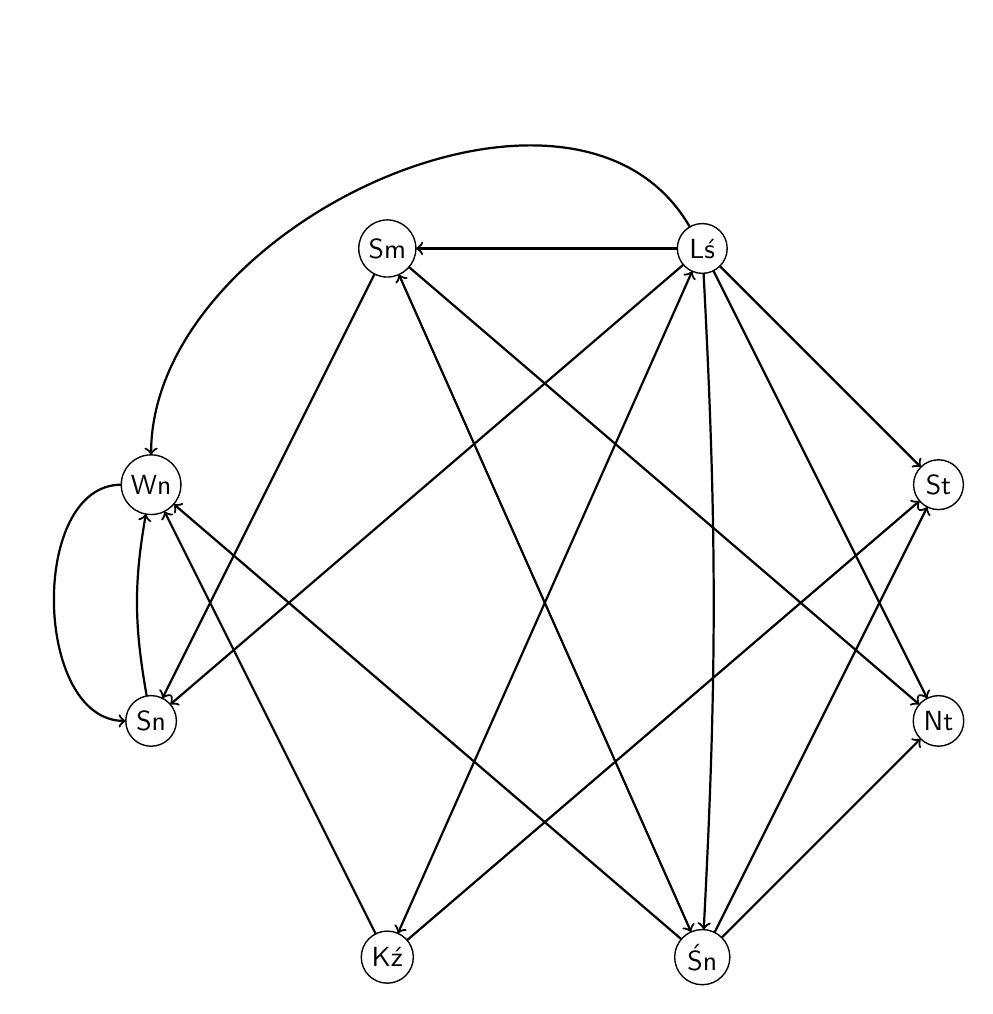
\begin{tikzpicture}
  \Vertex[x=3, y=9]{Sm}
  \Vertex[x=0, y=6]{Wn}
  \Vertex[x=0, y=3]{Sn}
  \Vertex[x=3, y=0]{Kź}
  \Vertex[x=7, y=9]{Lś}
  \Vertex[x=10, y=6]{St}
  \Vertex[x=10, y=3]{Nt}
  \Vertex[x=7, y=0]{Śn}
  \tikzset{EdgeStyle/.style={->}}
  \Edge[label=\tafSi](Sm)(Sn)
  \Edge[label=\txCoz](Sm)(Nt)
  \tikzset{EdgeStyle/.style={->,relative=false,in=180,out=180}}
  \Edge[label=\tafBr](Wn)(Sn)
  \tikzset{EdgeStyle/.style={->,relative=false,in=260,out=100}}
  \Edge[label=\tamSi](Sn)(Wn)
  \tikzset{EdgeStyle/.style={->}}
  \Edge[label=\txCoz](Kź)(St)
  \Edge[label=\tamBr](Kź)(Wn)
  \Edge[label=\txCoz](Lś)(Sm)
  \tikzset{EdgeStyle/.style={->,relative=false,in=90,out=120}}
  \Edge[label=\txCoz](Lś)(Wn)
  \tikzset{EdgeStyle/.style={->}}
  \Edge[label=\txCoz](Lś)(Sn)
  \Edge[label=\tamSi](Lś)(St)
  \tikzset{EdgeStyle/.style={->,relative=false,in=87,out=273}}
  \Edge[label=\tamSi](Lś)(Śn)
  \tikzset{EdgeStyle/.style={->}}
  \Edge[label=\tafSi](Lś)(Nt)
  \Edge[label=\txCoz](Śn)(Wn)
  \Edge[label=\tamBr](Śn)(St)
  \Edge[label=\tafBr](Śn)(Nt)
  \tikzset{EdgeStyle/.style={<->}}
  \Edge[label=\txCoz](Sm)(Śn)
  \Edge[label=\txCoz](Kź)(Lś)
\end{tikzpicture}
\end{center}

出于美观考虑,上图中所有的名字顶点均使用缩写,两个字母是名字的两个音节的首辅音字母。

八个点被分为两组,第一组为 \word{\Hoowen}、\word{\Hooyon}、\word{\Huuwen} 和 \word{\Huuyon},
第二组为 \word{\Teewen}、\word{\Teeyon}、\word{\Tiiwen} 和 \word{\Tiiyon}。
\word{\txCoz} 关系只出现在组间,其余同辈关系均出现在组内。

小组按什么规则进行划分的呢?已知的唯一一对亲兄弟姐妹,\word{\Hoowen} 和 \word{\Hooyon},出现在同一组。
可以判断出,这一组剩下的两人,也是亲兄弟姐妹,而且同性两人的子女会被分为一组——
如果是异性的话,无法确定分组:为什么一个男人的子女,要和他的姐姐(妹妹)的子女分为一组,
而不是和他的妹妹(姐姐)的子女分为一组?

根据前面关于父辈的讨论,\word{\Tee} 和 \word{\Tii} 为父辈的那对兄弟或姐妹。
牵涉到两者的表示异辈关系的词分别有 \word{\tFaSi}、\word{\tMoSi} 和 \word{\tangMo}。
虽然 \word{\tFaSi} 也为第一种声调,但与 \word{\Tii} 有此关系的 \word{\Huuyon},
却是和 \word{\Hoowen} 为一组,后者的父亲或母亲为 \word{\Hoo},与 \word{\Tii} 异性。
因此,\word{\Tii} 不可能是 \word{\Huuyon} 的父亲或母亲。因此,
\word{\tangMo} 是另外一个表示亲生关系的词。

那么,\word{\tangMo} 和 \word{\tangFa},谁代表父亲,谁代表母亲呢?我们可以发现,
\word{\tangMo} 的发音,类似各种语言中的母亲的发音,因此,\word{\tangMo} 代表母亲,
\word{\tangFa} 代表父亲。每组剩下的一对男女的父母也随之确定。

之前我们无法分辨 “\word{A B ’yn¹ X ngu².}” 表示的是 “A 是 B 的 X” 还是 “B 是 A 的 X”。
但在描述父亲关系的词中,父亲出现在 A,因此,我们可以断定这个句式表示的是 “A 是 B 的 X”。

现在,我们已经知道的有:

一、父辈四个人的性别。

二、子辈八个人的父母。

三、子辈中,\word{\Huuyon} 和 \word{\Hooyon} 同性;\word{\Tiiyon} 和 \word{\Teeyon} 同性。

稍作观察即可发现,描述同一组内亲属关系的共有四个词,分别是 \word{\tamBr}、\word{\tamSi}、
\word{\tafBr} 和 \word{\tafSi}。考虑到在 “A 是 B 的 X” 这样的表述中,
根据 A 和 B 性别不同,总共有四种可能,可以确定,这四个词对 A 与 B 的性别均有要求。
由于 \word{\tamBr} 用于两位男性之间,类似汉语中的关系\sq{兄弟},我们可以确定子辈八人的性别,并推出下表:

\begin{tabular}{c|c|l}
\hline
A & B & X \\
\hline
男 & 男 & \word{\tamBr} \\ \hline
女 & 男 & \word{\tamSi} \\ \hline
男 & 女 & \word{\tafBr} \\ \hline
女 & 男 & \word{\tafSi} \\ \hline
\end{tabular}

需要注意,本推理过于严谨,在实际做题的时候,没有必要。比如说,\word{\txCoz} 出现了十次,
又和 \word{\Hoo} 无关,便可以肯定这是描述子辈之间的一种极为松散的关系,且双方父母不同,
亲属关系较远,因为只有这样,才没必要分的十分仔细。

这是一道大约能在一个半小时完成的题目,有趣又不难。

\subsection{拓展阅读}

戴谊凡先生在闭幕式的说明中提到,西夏语的亲属系统很像塞内卡语的亲属系统。
下面给出了塞内卡语亲属系统的一组数据\cite{Seneca}。塞内卡语属于易洛魁语系,
在纽约州,还剩一百人使用这门语言。

表格的举例列使用缩写标记表达亲属关系:

F = Father, M = Mother, S = Sister, B = Brother, s = son, d = daughter.

标记应当从左往右当作一串亲属关系描述来理解,比如说 “FMSs”,就表示父亲的母亲的姐姐的儿子。

\sq{堂表}是指堂或表兄弟姐妹。

\begin{center}
\begin{tabular}{|c|c|p{10cm}|}
\hline
塞内卡语 & 汉语翻译 & \parbox[t]{10cm}{\centering{举例}} \\ \hline
\word{haʔnih} & 我的父亲 & F, FB, FMSs, FFBs, FMBs, FFSs, FFFBss \\ \hline
\word{noʔyẽh} & 我的母亲 & M, MS, MMSd, MFBd, MMBd, MFSd, MMMSdd \\ \hline
\word{hakhno ́ʔsẽh} & 我的叔叔 & MB, MMSs, MFBs, MMBs, MFSs, MMMSds \\ \hline
\word{ake:hak} & 我的阿姨 & FS, FMSd, FFBd, FMBd, FFSd, FFFBsd \\ \hline
\word{hatsiʔ} & 我的哥哥 & 
\parbox[t]{10cm}{B, MSs, FBs, MMSds, FFBss, MFBds, FMSss, MMBds\\比自己大} \\ \hline
\word{heʔkẽ:ʔ} & 我的弟弟 & 同上,但比自己小 \\ \hline
\word{ahtsiʔ} & 我的姐姐 & 
\parbox[t]{10cm}{S, MSd, FBd, MMSdd, FFBsd, MFBdd, FMSsd, MMBdd\\比自己大} \\ \hline
\word{kheʔkẽ:ʔ} & 我的妹妹 & 同上,但比自己小 \\ \hline
\word{akyã́:ʔse:ʔ} & 我的堂表 & 
\parbox[t]{10cm}
{MBs, FSs, MMSss, FFBds, MFBss, FMSds, MMBss\\
也可以是:\\
MBd, FSd, MMSsd, FFBdd, MFBsd, FMSdd, MMBsd} \\ \hline
\word{he:hawak} & 我的儿子 & 
\parbox[t]{10cm}{自己为男性:\\s, Bs, MSss, FBss, MBss, FSss, MMSdss} \\ & &
\parbox[t]{10cm}{自己为女性:\\s, Ss, MSds, FBds, MBds, FSds, MMSdds} \\ \hline
\word{khe:hawak} & 我的女儿 & 
\parbox[t]{10cm}{自己为男性:\\d, Bd, MSsd, FBsd, MBsd, FSsd, MMSdsd} \\ & &
\parbox[t]{10cm}{自己为女性:\\d, Sd, MSdd, FBdd, MBdd, FSdd, MMSddd} \\ \hline
\word{heyẽ́:wõ:tĕʔ} & 我的侄子 & 
\parbox[t]{10cm}{自己为男性:\\Ss, MSds, FBds, MBds, FSds, MMSdds} \\
\word{hehsṍʔneh} & &
\parbox[t]{10cm}{自己为女性:\\Bs, MSss, FBss, MBss, FSss, MMSdss} \\ \hline
\word{kheyẽ́:wõ:tĕʔ} & 我的侄女 & 
\parbox[t]{10cm}{自己为男性:\\Sd, MSdd, FBdd, MBdd, FSdd, MMSddd} \\
\word{khehsṍʔneh} & &
\parbox[t]{10cm}{自己为女性:\\Bd, MSsd, FBsd, MBsd, FSsd, MMSdsd} \\ \hline
\end{tabular}
\end{center}

很容易看出,塞内卡语的亲属关系和西夏语很接近。读者可以尝试分析并准确的定义每一个塞内卡语亲属关系,
找出其内在规律。
\section{第四题}

\def \oldman {老汉}
\def \man {男人}
\def \young {青年}
\def \child {儿童}
\def \woman {女人}
\def \girl {姑娘}
\def \thief {小偷}
\def \pig {猪}

\def \frighten {吓到}
\def \resemble {长得像}
\def \kill {杀}
\def \heal {治好}

\def \deceived {受骗}
\def \beaten {挨了打}
\def \evil {邪恶}
\def \coughing {咳嗽}

\def \null {null}
\newcommand \refer [2]{#1$_{\mbox{\tiny{#2}}}$}
\newcommand \getGender [1]{\ifx#1\woman 她\else\ifx#1\girl 她\else 他\fi\fi}
\newcommand \getPastTense [1]{\ifx#1\resemble 长 (过去时) 得像\else #1了\fi}
\newcommand \getFutureTense [1]{会 (将来时) #1}
\newcommand \notPastTense [1]{\ifx#1\resemble 长 (过去时) 得不像\else 没有#1\fi}
\newcommand \notFutureTense [1]{不会 (将来时) #1}
\newcommand \verbGen [2]{\ifcase #1\or \getPastTense{#2}\or 
\getFutureTense{#2}\or \notPastTense{#2}\or \notFutureTense{#2}\fi}
\newcommand \getPeople [3]{\ifx#2\null [这]\else 这一个\fi\ifx#3\null \else #3的\fi#1}
\newcommand \genHans [8]{\getPeople{#1}{#2}{#3}\verbGen{#4}{#6}#7吗?\\
\ifx#8\null \getPeople{#1}{#2}{#3}\else #8\fi
说\refer{\getGender{#1}}{\getPeople{#1}{#2}{#3}}\verbGen{#5}{#6}#7.}

\newcommand \didial [3]{\bipa{#1?} \bipa{#2.}\\#3}

以下为恩盖尼语的几段短篇对话及其汉语翻译:

\newcounter {exx}[section]
\newcounter {savexx}

\begin{enumerate}\setlength{\itemsep}{1pt}
\item \didial {edèì âno nw\d{á}sesè ozyí l\d{e}lemù à}
{edèì ânò wei ga òkí nw\d asese ozyí l\d{e}lemù}
{\genHans{\man}{this}{\null}{2}{4}{\frighten}{[这]受骗的小偷}{\null}}

\item \didial {\d{a}vùràmù k\d{i}nono amemùrè ânò à}
{\d{a}vùràmù wei ga òkì k\d{i}nono amemùrè ânò}
{\genHans{\woman}{\null}{\null}{1}{1}{\resemble}{这一个姑娘}{\null}}

\item \didial {\d{a}mó l\d{e}lemù \d{â}nó wuese \d{a}vùràmù à}
{\d{a}modhyòmù wei ga ò wuese \d{a}vùràmù}
{\genHans{\child}{this}{\deceived}{3}{1}{\kill}{[这]女人}{[这]青年}}

\item \didial {edèí dhia gbúnonò \d{a}mò à}
{\d{a}vùràmú kofilomù wei ga o gbúnonò \d{a}mò}
{\genHans{\man}{\null}{\evil}{2}{2}{\heal}{[这]儿童}{[这]咳嗽的女人}}

\item \didial {amemùré dhiá k\d{i}nono opilopo ânò à}
{\d{a}vùràmù wei ga \d{ó} k\d{i}nono opilopo ânò}
{\genHans{\girl}{\null}{\evil}{3}{3}{\resemble}{这一头猪}{[这]女人}}

\item \didial {ozyì gbunono okàá n\d{u}amù \d{â}nò à}
{ozyì wei ga òkí gbunono okàá n\d{u}amù \d{â}nò}
{\genHans{\thief}{\null}{\null}{1}{3}{\heal}{这一个挨了打的老汉}{\null}}

\item \didial {ozyi âno k\d{í}nonò edèí kofilomù à}
{\d{a}mò \d{â}nò wei ga \d{ó} k\d{i}nono edèí kofilomù}
\genHans{\thief}{this}{\null}{2}{4}{\resemble}{[这]咳嗽的男人}{这一个儿童}

\setcounter{exx}{\value{enumi}}\setcounter{savexx}{\value{enumi}}
\end{enumerate}
%
\begin{assgts}
\item 翻译成汉语:

\begin{enumerate}\setcounter{enumii}{\value{exx}}
\item \bipa{edèì ânò nw\d asese ozyi à?} \bipa{amemùrè wei ga \d{ò} nw\d asese ozyi.}
\item \bipa{amemùré l\d{e}lemu dhúnenè \d{a}modhyòmù \d{â}nò à?}\\
\bipa{amemùré l\d{e}lemu wei ga òki dhúnenè \d{a}modhyòmù \d{â}nò.}
\setcounter{exx}{\value{enumii}}
\end{enumerate}

这里还有恩盖尼语的一个答句, 但相应的问句没有给出:

\begin{enumerate}\setcounter{enumii}{\value{exx}}
\item \bipa{ozyi ânò wei ga \d{a}mó gbunono edèì.}
\setcounter{exx}{\value{enumii}}
\end{enumerate}

翻译成汉语. 如果译法不止一种, 请全部写出, 并解释你这样翻译的理由.

\item 翻译成恩盖尼语:

\begin{enumerate}\setcounter{enumii}{\value{exx}}
\item \genHans{\man}{\null}{\evil}{2}{2}{\heal}{[这]儿童}{[这]咳嗽的女人}{这一个咳嗽的青年}{[这]儿童}
\item \genHans{\woman}{this}{\beaten}{3}{3}{\frighten}{[这]男人}{\null}
\end{enumerate}

\item 假设你要编写一部恩盖尼词典, 那么表示 ‘小偷’ 和 ‘姑娘’ 的词的基本形式分别是什么? 解释你的答案.
\end{assgts}

恩盖尼语属于贝努埃-刚果语系。 在尼日利亚,只剩下二万人使用该语言。一个词的首个元音下面的标记 . 表明该词的所有元音发音时舌位都要稍微降低。标记 ˊ,ˋ, ˆ 分别表示高、低、降调;
如果以上标记均不出现,这个音节就发中调。

本题作者是阿尔图尔·谢梅纽克斯,他是 IOL 2012 第一题的作者。这题的排版怪坑的——把注释放在第二页。
赛前我校对过此题,知道音调标记,但没有注意到舌位降低的标记。影子赛中,我就直接把小点给无视了……

除了这个点,我感觉这题还是很简单的——我在填那份没人阅览的问卷调查的时候,最简单的题目选的就是它。

\subsection{推理过程}

事先声明,对于会发生变化的音调符号,独立于语境的引用,均省略音调符号,这不代表中调。

不知道这篇随笔的读者有没有新手。对于这种题,第一步做法永远是标出相同的名词或者动词。举个例子,
第二句和第三句都出现了\sq{\woman},也都出现了 \word{\d{a}vùràmù},因此,这个词极有可能是\sq{\woman}。
词可能会受时态、单复数等的影响,发生形态变化,因此,长得接近的词,比如说 \word{edèì} 和
 \word{edèí} 也极有可能是一个词。需要注意的是,当词或词缀很短的时候,这样的归类应当谨慎,
比如说今年第一题,一个辅音的变化就能表示不同的动词。

简单的分析可以发现,语序是 \textsf{SVO},问句句尾有 \word{à}。答句中,\word{wei ga} 表示\sq{说},
它的前面是说话人,后面跟着从句的主语——似乎是个代词,因为只有两种:\word{o} 和 \word{òki}。

对于名词,修饰语跟在名词的后面。\word{âno} 代表\sq{这一个}。

讨论一下 \word{o} 和 \word{òki}。这两个词作从句的主语,应当反应出从句主语的部分性质。简单归类可以发现,
\word{o} 表示说话者和从句主语一致,\word{òki} 表示不一致。第一小题的数据进一步验证了我们的猜想。

那么,如何表示时态与否定呢?我们已经确定,没有独立的单词表示否定或者时态。
\word{o} 和 \word{òki} 变化比较多,可能与之有关。列表:

\begin{tabular}{l|l|l}
\hline
\multirow{2}{*}{否定}
 & 过去 & 5. \word{ó}; 6. \word{òkí} \\ \cline{2-3}
 & 将来 & 7. \word{ó}; 1. \word{òkí} \\ \hline
\multirow{2}{*}{肯定}
 & 过去 & 3. \word{ò}; 2. \word{òkì} \\ \cline{2-3}
 & 将来 & 4. \word{o} \\ \hline
\end{tabular}

即,否定式,前词或主语(尚无法确定),末位元音高调,肯定过去时低调,肯定将来时中调。

我们同时可以注意到,每一句的动词在问句和答句中可能也会有变化。简单的前后对比可以发现,
在肯定将来时的情况下,动词的音调模式为:
\bgroup\glossfont
[\refer{V}{1}-\refer{V}{2}-\refer{V}{3}]→
[\refer{V́}{1}-\refer{V}{2}-\refer{V̀}{3}]
\egroup
,其余情况,动词所有音节均为中调。

\word{wei ga} 这两个词至少有一个表示动作\sq{说},但是两词均为中调,考虑到动作本身非否定,
我们可以推断,答句的主句也受同样的规则影响。我们发现,只有 \word{wei ga} 前的那一个单词,
可能是主语名词,也可能是名词修饰语,才会变调——比如说第四句的主语 \word{\d{a}vùràmú},
音调为高调,与肯定过去时不一致。

即动词只会让其前面的一个单词变调。

可以看出,恩盖尼语的变调相对复杂,这就给我们构建名词的原始形式造成了一定的困难——
这也是第三小题存在的意义。根据目前的推理,我们发现,宾语或者不与动词直接接触的主语均为原始形式。
然而,我们很快就发现了一个矛盾之处,第一句与第四句的主语 \word{edèi},音调不一致。
我们还可以发现第三句的宾语和第四句答句的主语 \word{\d{a}vùràmu},音调不一致。

这个时候就有两种观点,\word{à} 和 \word{âno} 让名词末位元音变成低调,
或名词后的形容词让名词末位元音变成高调。第一小题的第八句否决了前一猜想:
\word{à} 前的 \word{ozyi} 是中调。因此,形容词会导致名词变调。

最后,不要忘了舌位降低。我们发现,大部分舌位降低的词不存在未降低形式——我们可以假定舌位降低是这些词的自带属性——
但是 \word{o} 和 \word{ânò} 存在两种形式。分化条件相对简单,如果 \word{o} 后的动词舌位降低,
\word{o} 也会舌位降低;配合第六句,我们可以确定,\word{ânò} 前的词(不一定是修饰的名词)若舌位降低,
\word{ânò} 也会舌位降低。

至此,所有的点已被解决。

\section{第五题}

以下为西北格巴亚语的一些词和词组及其汉语翻译(乱序排列):

\begin{center}
\bipa{ʔáá, ʔáá náng nú kò, ʔáá sèè, búmá yík, búmá zù yík, dáng gòk, dí fò, dí sèè,\\
kò yík, kò zòk, náng wí, nú fò, nú lébé, sèè wí, yík, yík wí, zù}
\medskip

在……的表面; 眼窝; 眉毛; 睫毛; 眼睛/脸;\\
田边; 脚; 幸福; 肝; 良田; 鼻孔;\\
在……的上方; 毒蛇; 舌尖;\\
死 (动词); 嫉妒 (动词); 放 (动词)

\end{center}

\begin{assgts}
\item 将原文与译文正确对应起来.
\item 翻译成汉语: \bipa{búmá zù, kò, lébé gòk, lébé wí}.
\item 翻译成西北格巴亚语: 在……的中央; 头; 不愉快; 鼻子.
\end{assgts}

西北格巴亚语属于乌班吉语系。在中非共和国,尚有二十万人使用这门语言。

第五题是最难的一道题。本题的最佳解题奖给了来自上海外国语大学附属外国语学校的陈天陆,文科生。
她同时也是本届比赛中得分最高的中国队队员,以及 IOL 2014 Jeopardy 总分第三名。想要勾搭的同学们,加油!

鉴于我自己并没有认真做此题,所写的推理过程必受答案影响,我便邀请陈天陆分享她的推理过程,也让大家感受一下大神的气息。

\subsection{陈小姐的脑洞}
事先声明,陈天陆先将她的推理过程写在纸上,再拍下来发给我。我不得不手工完成再录入工作。与原稿相比,
文档布局基本不变,增加直角引号,重绘两个统计表格,并出于美观和卖萌考虑,将一处 “xx” 改为\sq{啥}。

如果大家感觉完全看不懂,或者太跳跃了,我在后面还附上了我精心构造的推理——虽然我是看过答案才写的。

\subsubsection{统计}
\begin{tabular}{c|c|l}
\hline
词数 & 次数 \\
\hline
1 & 3 & \word{ʔáá, yík, zù} \\
2 & 13 & 略 \\
3 & 1 & \word{búmá zù yík} \\
4 & 1 & \word{ʔáá náng nú kò} \\
\hline
\end{tabular}

\begin{tabular}{l|l}
\hline
次数 & 单词 \\
\hline
5 & \word{yík} \\
4 & \symfont{∅} \\
3 & \word{ʔáá, nú, kò, wí} \\
2 & \word{náng, sèè, búmá, zù, dí, fò} \\
1 & \word{dáng, gòk, sèè, zòk, lébé} \\
\hline
\end{tabular}

\subsubsection{猜}
最先猜出 \word{yík} =\sq{眼},因为出现频率最高,于是 \word{búmá zù yík} 和 \word{búmá yík} 分别对应睫毛和眉毛。
猜测\sq{睫毛}=\sq{眼的毛},\sq{眉毛}=\sq{眼上的毛},于是 \word{zù} 为\sq{在……的上方},
\word{kò yík} 是\sq{眼窝},\word{kò} =\sq{洞},\word{zòk} =\sq{鼻}。

剩下 \word{yík} 和 \word{yík wí},其中一个是\sq{眼}。考虑到:一、介词一般是单个词;
二、\sq{脸}$\approx$\sq{表面},\word{yík} =\sq{在……的表面},\word{wí} =\sq{身体部分}。
由此 \word{sèè wí} 和 \word{náng wí} 也是身体部分,推测一个是\sq{脚}一个是\sq{肝}(\sq{舌尖}不够基本)。

这时发现:

\newcommand \ctltable [3]{#1 = #2 & & #3 }
\begin{tabular}{rlll}
A & 的 & B & \\
\ctltable{幸福}{好}{肝} & 
\multirow{2}{10cm}{(还有一个原因是下题中要翻译\sq{在……中央}和\sq{不愉快},这让人联想到\sq{肝}是个重要的词)} \\
\ctltable{嫉妒}{啥}{肝} & \\
\ctltable{良田}{好}{田} &
\multirow{3}{10cm}{反正这就确定\sq{肝}= \word{sèè wí},那\sq{在……的中央}= \word{sèè},\word{náng} =\sq{脚}} \\
\ctltable{良田}{田}{边} & \\
\ctltable{舌尖}{舌}{边} & \\
\end{tabular}

这时候基本确定\sq{舌头} = \word{lébé},\word{dí} =\sq{好},\word{fò} =\sq{田},\word{nú}=\sq{边}。

然后看 \word{ʔáá náng nú kò},后三个词是\sq{脚+边+洞},听上去十分凶险,应该是\sq{死}……

不知道 \word{ʔáá} 和 \word{dáng gòk} 哪个是\sq{毒蛇},好像都解释得通,但下面有 \word{lébé gòk},
因为词能拆开,\word{dáng gòk} 应是 \sq{毒蛇},至此对应完毕。

\word{búmá zù} = 上面的毛 = 头发\\
\word{lébé gòk} = 蛇舌\\
\word{lébé wí} = 舌

头 = \word{zù}\\
不愉快 = 毒肝 = \word{dáng sèè}\\
鼻 = \word{zòk wí}

\subsection{我编出来的推理}

先看汉语。\sq{眼窝}、\sq{眉毛}、\sq{睫毛}和\sq{眼睛},都是和眼睛有关的东西。
汉语中还出现了\sq{在……的表面}与\sq{在……之上},而眉毛,就在眼睛的上方。
因此,这是一个很好的突破口。

\begin{tabular}{l|l}
\hline
次数 & 单词 \\
\hline
5 & \word{yík} \\
4 & \symfont{∅} \\
3 & \word{ʔáá, nú, kò, wí} \\
2 & \word{náng, sèè, búmá, zù, dí, fò} \\
1 & \word{dáng, gòk, sèè, zòk, lébé} \\
\hline
\end{tabular}

可以看到,出现了四次及以上的单词只有 \word{yík} 一个,其必然与眼睛有关。五个由其组成的短语中,
\word{yík} 位于词尾的有三个,即 \word{búmá yík}、\word{búmá zù yík} 和 \word{kò yík},
剩下为 \word{yík wí} 和 \word{yík}。鉴于 \word{búmá} 出现两次,可以推出其与毛有关,
构成的两个短语为\sq{眉毛}和\sq{睫毛},\sq{睫毛} 是眼睛的毛,\sq{眉毛} 在眼睛上方,
\word{zù} 也恰好独立出现过一次,应该就是\sq{在……的上方}。

亦可看出,\word{A B} 在西北格巴亚语中类似 “B 的 A”,因此 \word{kò yík} 是\sq{眼窝}(\sq{鼻孔}),
\word{kò} 可能是\sq{洞},也可能是\sq{在……的边上}(\sq{田边},眼窝可以看作眼球立体的边界)。

\word{kò} 出现在词首只有两次,另一次是 \word{kò zòk},若其代表\sq{在……的边上},
则 \word{zòk} 代表\sq{田},可后者只出现过一次,而\sq{田}还在\sq{良田}中出现过。
因此,\word{kò} 是\sq{洞},\word{kò zòk} 是\sq{鼻孔}。

回到 \word{yík wí},\word{wí} 这词还出现了两次,均在词尾。尚未确定的器官还有
\sq{肝}、\sq{脚} 和 \sq{舌尖}。\sq{舌尖} 看上去更是一个复合词,
因此 \word{wí} 位于词尾可能表示独立的器官。

现在我们还剩下以下词组:

\begin{enumerate}
\item \word{\hlc{ʔáá}, \hlc{ʔáá} náng nú kò, \hlc{ʔáá} sèè}

\item \word{\hlb{dí} \hla{fò}, \hlb{dí} sèè, \hlb{nú} \hla{fò}, \hlb{nú} lébé}

\item \word{dáng gòk}
\end{enumerate}

较为复杂的动词或动词短语,其语素或构成成分,至少有一个动词成分(词缀或中心词),如\sq{快走}里的\sq{走},
以及第三届全国语言学奥赛初赛第一题。这个动词成分的位置一般固定,如\sq{快走}和\sq{慢走}。考虑到 \word{ʔáá} 出现了三次,
均出现在词首,有理由相信这三个词对应着三个动词。

第二组词组中,\hlb{\word{dí}} 和 \hlb{\word{nú}} 各出现两次,均出现在词首。\hla{\word{fò}} 将这两类词连接起来。
对中文翻译分类,可以将\sq{幸福}和\sq{良田}分为一组(与\sq{好}有关),将\sq{田边}和\sq{舌尖}分为一组
(与\sq{在……的边上}有关),\sq{田}将这两类词连接起来。有理由相信,\hla{\word{fò}} 就是 \sq{田},我们只需判断,
\hlb{\word{dí}} 和 \hlb{\word{nú}},谁是\sq{好},谁是\sq{在……的边上}。

\word{\hlb{dí} sèè} 是一个引人注目的词,\word{sèè} 与 \word{wí} 构成一个短语,尚不知是\sq{肝}还是\sq{脚}。
我们知道,内脏,如\sq{心},在很多语言中表示心情。因此 \word{\hlb{dí} sèè} 应当就是\sq{幸福},
\word{sèè wí} 是\sq{肝},\word{náng wí} 是\sq{脚}。剩下的词也就随之确定了:

\begin{tabular}{c|c}
\hline
词组 & 翻译 \\
\hline
\word{dí} & \sq{好} \\
\word{nú} & \sq{在……的边上} \\
\word{dí fò} & \sq{良田} \\
\word{nú fò} & \sq{田边} \\
\word{nú lébé} & \sq{舌尖} \\
\word{dáng gòk} & \sq{毒蛇} \\
\hline
\end{tabular}

回到动词。\sq{放}在三个动词最为原始,我猜它就是 \word{ʔáá},这样一来:

\begin{tabular}{c|c|c}
\hline
词组 & 直译 & 翻译 \\
\hline
\word{ʔáá náng nú kò} & 放脚于洞边 & 死 \\
\word{ʔáá sèè} & 放肝 & 嫉妒 \\
\hline
\end{tabular}

\word{yík} 是\sq{在……的表面}。解决了两道小题的读者会发现,在西北格巴亚语中,方位词和器官词一致,
独立表示器官时需要加上 \word{wí},后者意为\sq{人}。许多非洲语言都有这一特征。


\renewcommand \refname{引用}
\bibliography{main}
\end{document}
